\documentclass[UTF8]{ctexart}
\usepackage{geometry}
\usepackage{amsmath}
\usepackage{graphicx} %插入图片的宏包
\usepackage{float} %设置图片浮动位置的宏包
\geometry{a4paper,scale=0.8}
\sectionfont{\bfseries\Large\raggedright}

\title{machine learning笔记}
\author{徐世桐}
\date{}
\begin{document}
\maketitle

% ----------------------------------------------------------------------
% |                              基础定义                               |
% ----------------------------------------------------------------------
\section{基础定义}
\noindent \textbf{二元分类}:输出分类个数为2\\
\textbf{多元分类}:输出分类个数不限

  $one-versus-the-rest$ OvR:计算属于每一分类的可能性,取可能性最大的分类为输出分类

  $one-versus-one$ OvO:对所有分类两两使用二元分类,每一分类器训练只需一部分数据\\
\textbf{multilabel多标签分类}:目标检测,对一图像中的物体加label\\
\textbf{multioutput多类分类}:多标签分类,每一标签可包含多种信息\\
\textbf{learning schedule}:根据迭代次数更新学习率\\
\textbf{early stopping}:提早结束训练

  对于每一epoch,当验证集MSE值增高时,证明开始overfit,停止训练

  即在epoch-error图中泛化误差最低时停止训练\\
\textbf{semi-supervised learning}: 部分样本有对应标签\\
\textbf{weakly-supervised learning}: 对样本标记包含的物体,而不标注对应目标的具体位置\\
\textbf{non parametric model}: 无法用有限的distribution parameter代表的模型,如Nearest neighbour\\
\textbf{在训练中使用正则化代价函数,训练结束后测试中代价函数不使用正则化项}\\
\textbf{curse of dimentionality}

  令$d$为特征数,$e$为一特征覆盖范围

  为了在$n$总样本中覆盖$k$个样本,平均需要e满足$e^d = \frac{n}{k}$

  随d升高,e值接近1。即每一特征需覆盖大部分取值范围使得k样本每个参数能同时被d个特征覆盖

  其余n-k样本存在特征取值范围的边界上,即\textbf{距离k样本距离几乎相同远}

% ----------------------------------------------------------------------
% |                              数学计算                               |
% ----------------------------------------------------------------------
\section{数学计算}
\noindent \textbf{MSE} = $\frac{1}{m}\sum_{i=1}^{m}(x^{(i)} - \bar{x} )^2$\\
\textbf{rigid regression}:回归方法,$J(\theta) = MSE(\theta) + \frac{\alpha}{2}\sum_{i}\theta_i^2$

  降低所有权重值\\
\textbf{lasso regression}:回归方法,$J(\theta) = MSE(\theta) + \alpha \sum_i |\theta_i|$

  降低不重要的权重值\\
\textbf{elastic net}:回归方法,$J(\theta) = MSE(\theta) + \gamma\alpha \sum_i |\theta_i| + (1-\gamma)\frac{\alpha}{2}\sum_{i}\theta_i^2$\\
\textbf{Normal Equation}:$\hat{\theta} = (X^TX)^{-1}X^Ty$

  直接得到权重$\hat{\theta}$,适用于仅有一个输出值的模型

  $X$为 (批量大小, 参数个数)输入矩阵,$y$为(批量大小, )向量
  
  当$X^TX$无逆矩阵时,用psudo inverse$\hat{\theta} = X^+y$\\
\textbf{pseudo inverse}:

  对矩阵$X=USV^T$,pseudo inverse $X^+=VS^+U^T$。$S^+$求法:

  \quad 1.对所有$S$元素,接近0的值赋为0

  \quad 2.对所有非零元素取倒数

  \quad 3.取矩阵转置,得到$S^+$\\
\textbf{log loss}:代价函数

  $J(\theta) = -\frac{1}{|B|}\sum_{i=1}^{|B|}[y^{(i)}log(\hat{p}^{(i)}) + (1-y^{(i)})log(1-\hat{p}^{(i)})]$

  标签值$y^{(i)}$为离散1/0值,计算值$\hat{p}^{(i)} \in [0,1]$

  微分:** 推导 **
  
  \quad $\frac{d J(\theta)}{d \theta_j} = \frac{1}{|B|}\sum_{i=1}^{|B|}(\hat{p}^{(i)} - y^{(i)}) x_j^{(i)}$\\
\textbf{Hinge loss}:代价函数

  $HingeLoss(y, \hat{y}) = max(0, 1-y*\hat{y})$

  应用于SVM,$y \in \{0, 1\}$,$\hat{y} \in \mathbb{R} $
  
  代表当预测值$\hat{y}$和y同号,$\hat{y} \geq 1$,则预测值和标签匹配,代价$=0$。否则$y*\hat{y} < 1$。代价值上升\\
\textbf{Gaussian Radial Basis Function RBF}:一种similarity function

  $\phi_{\gamma}(x, l) = exp(-\gamma||x-l||^2)$

  \quad $l$为landmark,即$\phi_{\gamma}$由一样本$x_i$和一landmark的距离得来\\
\textbf{Lagrange multipliers method拉格朗日乘数法}

  将\ 有前提的多项式求最值\ 问题转化为\ 无前提多项式最值问题

  定义:

  \quad 对输入向量$W$,$g(W) \geq 0$为constrain。目标为在满足$g(W) \geq 0$的前提下取$f(W)$最值

  \quad Lagrange function $\mathcal{L} (W, \alpha) = f(W) - \alpha(g(W))$

  \quad \quad $\alpha$为需要求解的变量之一,参与最终计算$W$的值。

  \quad \quad 当有多个constrain $g^{(i)}(W)$时,$\vec{\alpha}$为向量,求偏导对每一$\vec{\alpha}^{(i)}$求导

  \quad \quad 只有当$\alpha \geq 0$ 或每一$\vec{\alpha}^{(i)} \geq 0$,结果才有效

  \quad \quad $\vec{\alpha}^{(i)} = 0$代表对应的constrain $g^{(i)}(W)$为一个support vector

  计算:
  
  \quad 对每一$W$的元素\ 和\ $\alpha$取偏导,即向量
  $\begin{bmatrix}
    \frac{d \mathcal{L}(W, \alpha)}{d w_1}  \\
    \frac{d \mathcal{L}(W, \alpha)}{d w_n} \\
    ... \\
    \frac{d \mathcal{L}(W, \alpha)}{d w_n} \\
    \frac{d \mathcal{L}(W, \alpha)}{d \alpha}
  \end{bmatrix}$,计算向量$=\vec{0} $时的$W$, $\alpha$取值\\
\textbf{Distance Metrics}

  Manhattan distance(L1-norm): $d(x^{(i)}, x^{(j)}) = \sum_k |x^{(i)}_k - x^{(j)}_k|$

  Euclidean distance(L2-norm): $d(x^{(i)}, x^{(j)}) = \sqrt{\sum_k (x^{(i)}_k - x^{(j)}_k) ^ 2}$

  Chebyshev distance(L$\inf$-norm): $d(x^{(i)}, x^{(j)}) = \max_k |x^{(i)}_k - x^{(j)}_k|$\\
\textbf{information entropy}

  对单一一组数据$X = [x_1, ... x_n]$,$x_i$在$X$中出现百分比为$p(x_i)$
  
  $X$的数据熵$H(X) = -\sum_i p(x_i)log_2(p(x_i))$

  当$x_i$为continuous,不为离散值时,$X$即一分部。此时$H(X) = -\int_{x} p(x)log_2(p(x))\,dx $
% ----------------------------------------------------------------------
% |                             分类模型                                |
% ----------------------------------------------------------------------
\section{分类模型}
\noindent \textbf{classification}:

  binary classification: 拥有2类标签

  Multi-class classification: 拥有多类标签

  Milti-lable classification: 单个样本可以属于多个标签\\
\textbf{logistic regression}:

  判断输入符合每一输出类别的可能性,

  分类:

  \quad Simple regression:单个样本变量个数为1

  \quad Multiple regression:样本变量个数 > 1

  \quad Mutivariate regression: 单个样本对应标签个数 > 1

  前向计算:
  
  \quad 1.$\hat{p} = \sigma(\theta^Tx + b)$

  \quad 2.$\hat{y} = 1\space (if \hat{p} \geq 0.5)$

  \quad \quad \quad $= 0\space (if \hat{p} < 0.5)$

  代价函数为log loss\\
\textbf{SVM}

  找到分界,分离多种数据

  support vector: 最靠近分界线的样本

  hard margin classification硬性分类:限制数据必须被分界隔开,同一类数据不可同时出现在分界2端

  soft margin classification:与硬性分类相反,避免被outlier离群值影响

  前向计算:$\hat{p} = f(x_1, x_2,...)$,其余同logistic regression

  \quad 区别:$f$可为polynomial,非线性函数。可使用kernel trick

  线性分类训练:$\hat{p} = W^Tx + b$,$W$ 为参数\textbf{向量}

  \quad \textbf{硬性分类}:

  \quad \quad $||W||_2$代表线性函数斜率

  \quad \quad 最小化$\frac{1}{2}W^TW$,使得分界平面的斜率最小,最大化分界线和两种数据的距离

  \quad \quad 前提:对每一样本$i$, $1.y^{(i)}\hat{p}^{(i)} \geq 1$,即标签和计算结果相同

  \quad \quad 求解:1.直接解以上带前提的不等式

  \quad \quad \quad '当样本数高于参数数量时使用,由于dual form的复杂度为$O(|S|^2)$ - $O(|S|^3)$,直接解复杂度为$O(|S|)$'
  
  \quad \quad 2.使用拉格朗日乘数法得到dual form,其中$\vec{\alpha}$为向量。$\textbf{x}^{(i)}$为第i样本的特征值向量$\mathcal{L} = \frac{1}{2}W^TW - \sum_{i=1}^{|B|}\vec{\alpha}^{(i)}(y^{(i)}\hat{p}^{(i)} - 1)$

  \quad \quad \quad 使偏导向量为$\vec{0} $,得到$2.W = \sum_{i=1}^{m}\vec{\alpha}_iy^{(i)}\textbf{x}^{(i)}$, $3.\sum_{i=1}^{m}\vec{\alpha}_iy^{(i)}=0$

  \quad \quad \quad 带入得$\mathcal{L} (W, \vec{\alpha}) = \frac{1}{2}\sum_{i=1}^{|B|}\sum_{j=1}^{|B|}\vec{\alpha}_i\vec{\alpha}_jy^{(i)}y^{(j)}\textbf{x}^{(i)^T}\textbf{x}^{(j)} - \sum_{i=1}^{|B|}\vec{\alpha}^{(i)}$
  
  \quad \quad \quad \quad $=\frac{1}{2}\vec{\alpha}^T (\textbf{x} * y)(\textbf{x} * y)^T \vec{\alpha} - \sum_{i=1}^{|B|}\vec{\alpha}^{(i)}$

  \quad \quad \quad \quad 其中$(\textbf{x} * y)$为广播乘法\ 将训练集矩阵每一样本乘以对应标签值,$y$为标签列向量

  \quad \quad \quad 使用QP solver得到使$\mathcal{L} (W, \vec{\alpha})$最小,$\vec{a}^{(i)} \geq 0$的向量$\vec{\alpha}$

  \quad \quad \quad 解$W$:由$\vec{\alpha}$带入2.式计算,$\vec{\alpha}$已被clamp,见经验2.

  \quad \quad \quad 解$b$:由于所有support vector $\textbf{x}^{(i)}$ 满足1.式,则对所有support vector计算$b$取平均值

  \quad \quad \quad \quad $b = E_{a^{(i)} \geq 0}(y^{(i)}-W^T\textbf{x}^{(i)})$

  \quad \quad 3.直接进行梯度下降,代价函数$J(W, b) = \frac{1}{2}W^TW + const \sum_i HingeLoss(y^{(i)}, \hat{p}^{(i)})$
  
  \quad \textbf{软性分类}:

  \quad \quad 最小化$\frac{1}{2}W^TW + C\sum_{i=1}^{|B|}\zeta_i $

  \quad \quad \quad $\zeta_i$定义第$i$样本被忽视为误差样本的可能性,$C$定义忽视率相对斜率的权重

  \quad \quad 前提:对每一样本$i$,$y^{(i)}\hat{p}^{(i)} \geq 1 - \zeta^{(i)}$

  非线性分类方法:

  \textbf{- 使用polynomial做$f$}

  \quad 必须使用拉格朗日乘数法求解,目的为\textbf{对$\phi(x)$得到线性权重和偏差},求解使用dual form,其中包含$\phi(a)^T \cdot \phi(b)$项即可使用kernel method

  \quad 权重$W$公式不再适用,由于结果不为线性

  \quad 偏差$b = \sum_{\vec{\alpha}^{(i)} \geq 0} y^{(i)} - \sum_{\vec{\alpha}^{(j)} \geq 0} \vec{\alpha}^{(i)} * y^{(j)} * K(\textbf{x}^{(i)}, \textbf{x}^{(j)})$

  \textbf{- 使用similarity function}:
  
  \quad 选择多个landmark$\mathcal{L} = l_1, l_2, ..., l_n$,对每一样本$x_i$计算其和每一$l_j$的$\phi_{\gamma}$值$\phi_{\gamma}(x_i, l_j)$

  \quad 每个样本用新的向量$x_i' = \begin{bmatrix}
    \phi_{\gamma}(x_i, l_1) \\
    \phi_{\gamma}(x_i, l_2) \\
    ... \\
    \phi_{\gamma}(x_i, l_n)
  \end{bmatrix}$表示。新的向量组成训练集,进行SVM训练

  \textbf{kernel}:

  \quad 定义:能够从输入向量$a$,$b$,不通过计算$\phi(a), \phi(b)$直接得到点乘结果$\langle \phi (a), \phi (b)\rangle $的函数

  \quad 例:** 是否通过取linear 为phi得到kernel 函数 **

  \quad \quad linear: $f(a, b) = a^Tb$

  \quad \quad polynomial: $f(a, b) = (\gamma a^Tb+r)^d$

  \quad \quad \quad poly的$\phi(x)$为对向量x每一元素进行poly运算,结果向量元素数不变

  \quad \quad Gaussian RBF: $f(a, b) = exp(-\gamma ||a-b||^2)$

  \quad \quad Sigmoid: $f(a, b) = tanh(\gamma a^Tb + r)$

  \quad \textbf{经验总结}:

  \quad \quad 1.QP solver中需限定$\sum_{i=1}^{m}\vec{\alpha}_iy^{(i)}=0$,否则得出$\hat{\alpha}$不遵循此等式

  \quad \quad 2.当样本有重叠,仍可使用拉格朗日乘数法,异常样本被分入错误类别。

  \quad \quad \quad 此时$\vec{\alpha}$包含负值,对应的样本在计算权重\ 偏差时被忽略,即需clamp使$\vec{\alpha} \geq 0$

  \quad \quad \quad 若不进行clamp,得到的分界仅有略微差别,不会造成大幅误差。(在线性\ 非线性分类都有验证)

  \quad \quad 3.梯度下降直接得到最优$W, b$,无法通过梯度下降得到$\vec{\alpha}$ 由于梯度下降忽略限制条件

  \quad \quad 4.QP solver需要$(\textbf{x} * y)(\textbf{x} * y)^T$为positive definite,计算时加上对角矩阵$diag(\epsilon)$即可,$\epsilon$多取$10^{-4}$

  \quad \quad \quad 否则迭代解QP时出现KKT condition not met或positive definite条件不满足

  \quad \quad \quad 条件不满足时中断得到的$\vec{\alpha}$无法作为有效结果参与后续计算权重和偏差

  \quad \quad \quad 优先将此矩阵转为float64类型,否则需要$\epsilon$较大才能保证positive definite
  
% ----------------------------------------------------------------------
% |                               KNN                                  |
% ----------------------------------------------------------------------
\section{KNN}
\noindent lazy learner: 仅在得到特征后进行计算,得到训练集后仅仅保存训练集\\
  定义:

  \quad 得到样本集S,每次得到需要预测的特征向量$x$\\
  算法:

  \quad 从样本特征集中选取k个最邻近$x$的样本,距离由distance metric计算,返回k个样本标签中占比较大的标签\\
\textbf{distance weighted KNN}

  算法:

  \quad 对k个邻近样本,每一分配权重$w_i$。

  \quad 对k个样本中同一标签下的样本权重求和,总和较高的标签作为结果

  取$w_i$方法1:

  \quad 1. $w_i = \frac{1}{d(x^{(i)}, x)}$

  \quad 2. $w_i = \frac{1}{2\pi} exp(-\frac{d(x^{(i)}, x)^2}{2})$

  \quad $d(x^{(i)}, x)$来自distance metric

  优劣:

  \quad 1. k值影响较小,由于较远的样本$w_i$较小

  \quad 2. 受curse of dimentionality影响。可对每一特征加权重\ 或\ feature extraction解决\\
\textbf{KNN regression}

  样本标签不为离散值,而为连续值,求regression。

  算法:

  \quad 对所有可能的feature向量$x$,取距离$x$最近的k个样本。
  
  \quad $x$的标签值为k个样本的平均值。此值即为regression结果\\
\textbf{Locally weighted regression}

  distance-weighted KNN,将K个邻近样本的距离作为权重$w_i$。计算$x$标签$ = \sum_i w_i \cdot d(x^{(i)}, x)$



% ----------------------------------------------------------------------
% |                              决策树                                 |
% ----------------------------------------------------------------------
\section{决策树}
\noindent 定义:

  节点$N_i$:

  \quad 节点条件:判断样本进入哪一子节点,叶节点没有节点条件
  
  \quad sample属性$S_i$:有多少样本\textbf{进入$N_i$节点},非满足$N_i$节点条件的样本个数

  \quad value属性$V_i = v_{i1}, ..., v_{in}$:$S_i$进入节点的样本中$v_{ij}$个属于第$j$分类
  
  \quad 子节点仅有2个,对应节点条件为true/false的情况\\
分类方式:数据从根节点开始,根据节点条件传向对应子节点。直到到达叶节点。叶节点中$V$属性中最大项即数据分类\\
在imbalanced dataset上训练效果不好\\
\textbf{CART algorithm创建决策树}:

  根节点初始化为叶节点,没有节点条件
  
  对每一叶节点$S_i$选取一特征$k$,一特征门槛$t_k$,将样本集分为2组$S_{true}, S_{false}$。
  
  \quad 选取$(k, t_k)$方式:使代价函数$J(k, t_k) = \frac{S_{true}}{S_i}G_{true} + \frac{S_{false}}{S_i}G_{false}$最小

  \quad gini属性$G_i$:数据混杂度,$G_i = 1-\sum_{j=1}^{n}(\frac{v_{ij}}{S_i})^2$

  直到决策树层数达到固定上限,或对所有分组条件$(k, t_k)$,$J(k, t_k) \geq G_i$\\
\textbf{information gain创建决策树}

  允许单个节点$N_i$有多个子节点$C_i = {N_j}$,(在特征为离散分类时)

  选取子集方式:最大化information gain $IG(N_i, C_i) = H(N_i) - \sum_{N_j \in C_i}(\frac{S_j}{S_i}H(S_j))$
  
  \quad $H()$为information entropy,\textbf{替换CART法中的gini属性}
  
  所有特征为实数创建决策树:
  
  \quad 将$S_i$样本按照实数特征排序,随后选择特征\ 门槛$(k, t_k)$,将数据分为2组,最大化information gain

  \quad 即CART algorithm,使用不同数据混杂度函数
  
  所有特征为类别参数:
  
  \quad 选择类别特征$t$,$t$中每一类别对应一子节点。即$t$的值域=子节点数\\
\textbf{避免overfit}

  1.设置决策树层数上限

  2.设置节点样本下限,若样本数量低于下限则停止继续分类
  
  3.pruning\\
\textbf{使用决策树进行regression}

  \begin{figure}[H] %H为当前位置,!htb为忽略美学标准,htbp为浮动图形
    \centering %图片居中
    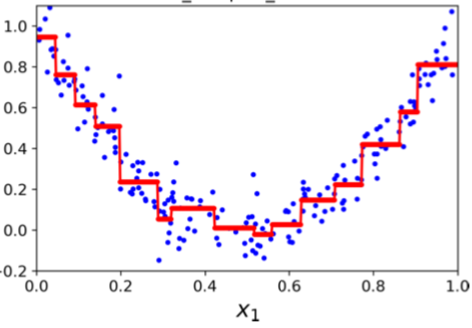
\includegraphics[width=0.3\textwidth]{note_images/deci_tree_regression.png} %插入图片,[]中设置图片大小,{}中是图片文件名
  \end{figure}

  输入样本,分类进不同值域

  更改:
  
  \quad 每一节点value值为一常数,为$S_i$样本的平均值。
  
  \quad 输出值为叶节点的value,非最大value对应的类别

  \quad $G_i$为$S_i$样本的方差$\frac{1}{S_i}\sum_{j=1}^{S_i}(x_i^{(j)} - \bar{x}_i)^2$

% ----------------------------------------------------------------------
% |                 ensemble learning random forest                    |
% ----------------------------------------------------------------------
\section{ensemble learning \& 随机森林}
\noindent \textbf{ensemble learning}:使用一组预测机制进行学习,预测机制可为不同算法

  dropout为一种ensemble learning,由于丢弃神经元即改变网络结构\\
\textbf{random forest随机森林}:

  训练方法:随机选择$n$个训练子集$s_1, s_2, ..., s_n \in S$,训练$n$个决策树$t_1, ..., t_n$。
  
  前向计算:对$n$个树产生的$n$个分类结果,选取投票最多的一分类作为结果
  
  训练子集选取:bagging:子集可重复选取一样本,pasting:样本不重复
  
  \quad out-off-bag oob 样本:当使用bagging选取时,平均只有$1-e^{-1}$样本被选择,余下样本被称为oob样本

  优化:

  \quad random patches随机贴片:对特征和训练集同时取子集进行训练
  
  \quad random subspace随机子空间:对特征取子集,对整个总训练集进行训练
  
  \quad extra-trees极度随机森林:'使用随机$t_k$而不使用最小化数据混杂度的$t_k$'
  
  \quad $k$feature importance特征重要性:对所有取$k$为判断条件的节点$N_i$,计算加权平均值$\sum_i(S_i$imprity降低百分比$)$
  
  \quad (hypothesis) boosting:合并多个预测机制据结果的方法
  
  \quad \quad AdaBoost:串联预测机制,对上一预测机制遗漏的样本加更高权重,进行训练

  \quad \quad gradient boosting


% ----------------------------------------------------------------------
% |                     dimentionality reduction                       |
% ----------------------------------------------------------------------
\section{维度下降}
\noindent 根据manifold assumption,高维空间中训练集参数点稀疏。则将数据压缩到低维\\
\textbf{principle component analysis PCA}:

  对训练集参数矩阵取SVD$USV^T$

  取$V$中前$d$个向量$V' = [v_1, ..., v_d]$,新训练集$A_{compressed} = A_{origin}V'$
  
  从\ 新训练集\ 延展回\ 原训练集纬度:$A_{expand} = A_{compressed}V'^T$\\
\textbf{Incremental PCA}:无需整个训练集存在内存中即可进行SVD\\
\textbf{kernel PCA}:**\\
\textbf{local linear Embedding LLE}:
  
  对每一样本$x^{(i)}$寻找$k$个相邻样本\ 相邻样本index的集合称$C_{x^{(i)}}$
  
  构建$(|S|, |S|)$矩阵$W$:
  
  \quad 每一行向量$[W_{i1}, ..., W_{i|S|}]$满足$x^{(i)} - \sum_{j \in C_{x^{(i)}}} W_{ij}x^{(j)}$
  
  \quad 每一行向量$W_i$求和为1:$\sum_{i=1}^{|S|}W_i = 1$

  由$W$创建新训练集:

  \quad 令$z^{(i)}$为$x^{(i)}$在低维的投影

  \quad 使所有$z^{(i)}$满足最小化$(z^{(i)} - \sum_{j=1}^{|B|}w_{ij}z^{(j)})^2$

% ----------------------------------------------------------------------
% |                             聚类分析                                |
% ----------------------------------------------------------------------
\section{聚类分析}
\noindent \textbf{K-mean}:

  将数据分为k个cluster,每个cluster有中心点称centroid
  
  算法:
  
  \quad 1.初始化随机选择k个样本位置做centroid,避免得到空cluster

  \quad \quad 当迭代过程中出现空cluster,从其他cluster中分配一随机参数点给此cluster

  \quad 2.分配样本:每个样本分入距离最近的centroid的cluster

  \quad 3.更新centroid:新centroid为cluster中样本坐标平均值。
  
  \quad 重复第2.3.步,直至centroid不再移动,或移动距离小于定值

  vornoid diagram:

  \quad 画有不同cluster的分界线的图

  迭代:
  
  \quad 多次随机初始化centroid,选择其中inertia最小的centroid取法进行训练

  \quad \quad interia = $\frac{1}{|S|}\sum_x (C_x - x)^2$。

  \quad \quad \quad $C_x$为样本x距离最近的centroid

  \quad k-mean++初始化centroid:

  \quad \quad 1.随机选择1个样本做centroid

  \quad \quad 2.剩余每一样本$x^{(i)}$有$\frac{D(x^{(i)})}{\sum_{j=1}^{|S|} D(x^{(j)})}$几率被选做新centroid

  \quad \quad \quad $D(x^{(i)})$为样本$x^{(i)}$距离最近的centroid的距离

  \quad \quad 3.重复2.步直至得到k个centroid

  \quad 选择cluster数量k:
  
  \quad \quad elbow approach:

  \quad \quad \quad 实验多次,每次选择不同k值。记录最终loss大小,k-loss图像应当最初快速减小,随后连线平缓。选择拐点处的k值作为最优超参数

  \quad \quad cross validation:

  \quad \quad \quad 数据分为n fold,得到n组训练集,验证集分配

  \quad \quad \quad 选择不同k值,对每一k值\ 在每一训练集上训练,在验证集得到验证代价值。共得到n*k验证代价

  \quad \quad \quad 取k使得平均验证代价值最小

  \quad \quad sihouette score:所有样本的sihouette coefficient的均值

  \quad \quad \quad 一样本$x^{(i)}$的sihouette coefficient:$\frac{b-a}{max(a, b)}$

  \quad \quad \quad \quad $a$为$x^{(i)}$到同一cluster内所有样本的平均距离
  
  \quad \quad \quad \quad $b = min(E_{x^{(j)} \in other \space cluster}(D(x^{(i)} - x^{(j)})))$

  \quad \quad \quad sihouette score$\in [-1, 1]$,偏向取score高的cluster数

  使用k-mean进行数据预处理:

  \quad 将数据首先进行k-mean分类,将每一样本替换为\ 样本到最近的centroid距离,传入另一模型进行学习

  \quad 用于半无监督学习:将数据进行k-mean分类,从每一cluster选取离centroid最近的样本,产生大小为k的训练集。则只需得到k个样本的标签即可进行训练\\
\textbf{k-mode}

  选择centroid使每一特征值分别为\ 对应特征中出现次数最多的特征值\\
\textbf{Probability Density Estimate PDE}

  得到样本分布的pdf:$\hat{p}$,对特征$x$输出可能性$\hat{p}(x)$

  non-parametic approach:不对数据的分部做任何假设
  
  \quad 根据整个训练集集$S$训练,lazy learning

  \quad kernel density estimation:

  \quad \quad 1.$\hat{p}(x) = \frac{1}{|S|}\sum_{x^{(i)} \in S}\frac{1}{h^D}H(\frac{x - x^{(i)}}{h})$

  \quad \quad \quad D为feature个数,h为bandwidth,$h^D$即window体积

  \quad \quad \quad H称Parzen Window/kernel function\begin{equation*}
    H(x) = \begin{cases}
    1 &\forall i \in \{1, ..., D\}, |x_i| < \frac{1}{2}\\
    0 & otherwise
    \end{cases}
  \end{equation*}
  
  \quad \quad \quad $H(\frac{x - \hat{x}^{(i)}}{h})$即判断$x$是否在给定数据$x^{(i)}$h大小 window内

  \quad \quad 2.$\hat{p}(x) = \frac{1}{|S|}\sum_{x^{(i)} \in S}\frac{1}{(2 \pi h^2)^{\frac{D}{2}}}exp(-\frac{||x - x^{(i)}||^2}{2h^2})$\\

  parametic approach:

  \quad Gaussian distribution:假设pdf为Normal分部

  \quad \quad \textbf{直接根据训练集得到最优参数,没有迭代}

  \quad \quad 1.univariate Normal distribution:仅有一特征
  
  \quad \quad \quad $\hat{p}(x) = N(x|\mu, \varSigma) = \frac{1}{\sqrt{2\pi \sigma^2}}exp(-\frac{(x - \mu)^2}{2\sigma^2})$

  \quad \quad \quad \quad $\mu = \frac{1}{|S|}\sum x^{(i)}$

  \quad \quad \quad \quad $\sigma^2 = \frac{1}{|S|}\sum(x^{(i)} - \mu)^2$

  \quad \quad \quad \quad 即multivariate Normal dis中$D$ = 1情况

  \quad \quad 2.multivariate Normal distribution:有多个特征
  
  \quad \quad \quad $\hat{p}({\bf x}) = N({\bf x}|\mu, \varSigma) = \frac{1}{\sqrt{(2\pi)^D|\varSigma|}}exp(-\frac{1}{2}({\bf x}-\mu)^T\varSigma^{-1}({\bf x}-\mu))$

  \quad \quad \quad \quad $|\varSigma|$项为$\varSigma$determinant

  \quad \quad \quad \quad $D$为特征数

  \quad \quad \quad \quad $\mu = \frac{1}{|S|}\sum_{x^{(i)} \in S}{\bf x}^{(i)}$

  \quad \quad \quad \quad covariance matrix $\varSigma = \frac{1}{|S|}\sum_{x^{(i)} \in S}({\bf x}^{(i)} - \mu)({\bf x}^{(i)} - \mu)^T$

  \quad \quad 计算performance:neg. log-likelihood

  \quad \quad \quad $\mathcal{L} = -log(p(S | \mu, \varSigma)) = -\sum_{x^{(i)} \in S} log(p({\bf x}^{(i)}|\mu, \varSigma))$

  \quad \quad Theorem:当neg. log-likelihood 最小化,$\mu$和$\sigma$有以上公式求解

  \quad \quad \quad \quad $= \frac{N}{2}log(2\pi) + \frac{N}{2}log(\sigma^2) + \frac{1}{2\sigma^2}\sum_{x^{(i)} \in S}(x^{(i)} - \mu)^2$

  \quad \quad \quad 当$\frac{d\mathcal{L}}{d\mu} = 0$和$\frac{d\mathcal{L}}{d\sigma^2} = 0$,$\mu$和$\sigma$有以上公式求解\\
\textbf{Gaussian Mixtures Model(GMM)}:一种PDE,假设所有子分部都为正态分部

  参数:$\theta = \{ \pi_k, \mu_k, \varSigma_k | k = 1..K\}$
  
  \quad \quad 共K个子分部,每一分部$\sim N(\mu_k, \varSigma_k)$
  
  使用多个子分部之和代表样本pdf分部,$p(x) = \sum_{k=1}^{K} \pi_kN(x|\mu_k, \varSigma_k)$

  \quad x可为向量,则$p(x)$计算方法同Multivariate Normal Distribution

  \quad \quad 此时称多元混合高斯分布
  
  \quad $0 \leq \pi_k \leq 1$, $\sum_{k=1}^{K}\pi_k = 1$,保证产生的pdf 积分为1

  迭代:

  \quad 1.随机初始化所有参数,仅保证$\sum \pi_k = 1$

  \quad 2.E-Step 

  \quad \quad 对每一样本i,子分部k计算responsibility $r_{ik} = \frac{\pi_kN({\bf x}^{(i)} | \mu_k, \varSigma_k)}{\sum_j^K\pi_jN({\bf x}^{(i)} | \mu_j, \varSigma_j)}$

  \quad 3.M-Step

  \quad \quad 定义$N_k = \sum_{i=1}^{|B|} r_{ik}$对一子分部的responsibility求和

  \quad \quad 更新$\mu_k = \frac{1}{N_k}\sum_{i=1}^{|B|}r_{ik}{\bf x}^{(i)}$

  \quad \quad 更新covariance matrix $\varSigma_k = \frac{1}{N_k}\sum_{i=1}^{|B|}r_{ik}({\bf x}^{(i)} - \mu_k)({\bf x}^{(i)} - \mu_k)^T$

  \quad \quad \quad 使用当前M-Step已更新的$\mu$

  \quad \quad 更新$\pi_k = \frac{N_k}{|B|}$

  \quad 4.当$\theta$不再大幅改变,\textbf{或当neg. log likelihood不再下降}则停止,否则回到2.

  \quad \quad neg. log likelihood $\mathcal{L} = -\sum_{x^{(i)} \in S} log(p({\bf x}^{(i)}|\mu, \varSigma))$

  \quad \quad \quad $p$ 为K个子分部加权求和值,即一样本输出的fit值

  调参:选择子分部个数K

  \quad $BIC_K = \mathcal{L}(K) + \frac{P_K}{2}log(|B|)$

  \quad \quad $\mathcal{L}(K)$为使用K类别时的neg. log likelihood

  \quad \quad 当使用特征个数n时,$P_K = n * \frac{(n+1)n}{2} * k - 1$为使用的参数个数

  \quad \quad \quad $n$对应使用的$\mu$个数

  \quad \quad \quad $\frac{(n+1)n}{2}$covariance 参数个数,由于$\varSigma$为n*n symmetric matrix

  区别K-mean:

  \quad GMM-EM 可得到一样本i属于每一类别k的可能性,即$r_{ik}$

  \quad GMM-EM cluster等高线可以为非正圆,K-mean每一cluster为正圆从centroid向外发散
  
  \quad GMM-EM cluster等高线集中程度可不同,K-mean每一cluster等高线间距相同
  
  \quad \quad \textbf{cluster间分界不受等高线的弧形影响,受交接的2子分部影响}\\
\textbf{DBSCAN}

  适用于一cluster内样本密度较高的训练集

  算法:

  \quad 1.对每一样本$x_i$计算集合$S_{i\varepsilon}$,称$\varepsilon -neighbourhood$,包含所有距离在$\varepsilon $内的其他样本

  \quad \quad $|S_{i\varepsilon}| > $超参数$s_{min}$\ 的样本称core instance

  \quad 2.所有属于同一$S_{i\varepsilon }$的样本判为属于同一cluster,当一样本$x_i$同时存在样本$x_i, x_j$的$\varepsilon -neighbourhood$中时,合并$S_{i\varepsilon }, S_{j\varepsilon }$。

  \quad 3.没有被分配进任何$S_{i\varepsilon }$的样本判为异常值

% ----------------------------------------------------------------------
% |                              对抗网络                                |
% ----------------------------------------------------------------------
\section{GAN对抗网络}
\noindent \textbf{基本结构}:

  generator $G$:得到正则噪声$\mathbf{z}$,生成伪数据$\mathbf{x}'$。目标为使$D(\mathbf{x}') = 1$
  
  discriminator $D$,从实际数据集$\mathbf{x}$或伪数据集$\mathbf{x}'$得到数据判断真伪。即对伪数据输出0\ 真数据1。

  一次训练:(首先进行D更新,后进行G更新)

  \quad \textbf{两部分使用不同trainer,每一部分计算代价值后立即更新参数}

  \quad 1.discriminator部分:
  
  \quad \quad 得到一批量正则噪声$\mathbf{z}$,计算伪数据$\mathbf{x}' = G(\mathbf{z})$,标签为$\vec{0}$。
  
  \quad \quad 取一批量真实数据$\mathbf{x}$,标签为$\vec{1}$。
  
  \quad \quad 对2批量数据分别使用二元交叉熵损失函数训练。最终代价值为两部分代价值平均值。

  \quad \quad 调用D部分的trainer

  \quad 2.generator生成数据

  \quad \quad 与D部分使用同一批量正则噪声,使用未更新的G参数和\textbf{已更新的G参数}前向计算。输出的标签期望为$\vec{1}$
  
  \quad \quad 即代价函数为$J_G = -y \space log(D(G(\mathbf{z})))$ 
  
  \quad \quad \quad $ = - \space log(D(G(\mathbf{z})))$ (y必为1,由于期望产生$\mathbf{x}'$使$D(\mathbf{x}') = \vec{1}$)
  
  \quad \quad 调用G部分的trainer\\
\textbf{Deep Convolutional GAN}


% ----------------------------------------------------------------------
% |                             RL强化学习                               |
% ----------------------------------------------------------------------
\section{RL强化学习}
\noindent \textbf{基本定义}

  程序在 environment环境中根据观测得到的 state状态,选择 action行为,得到reward反馈

  模型整体符号定义<A, S, R, P>

  \quad Action space $A$
  
  \quad State space $S$
  
  \quad Reward $R$: $\sum \times A \times S$ → $R$
  
  \quad Transition $P$: $\sum \times A$ → $S$

  第$i$决策的符号定义:

  \quad $a_i \in A$ 采取的行为

  \quad $r_i \in R$ 得到的reward,每一行为可以立即得到反馈值
  
  exploring探索:模型尝试新行为
  
  exploiting利用:模型使用已知高反馈行为\\
\textbf{policy}

  根据观测选择$a_i$的算法

  stochastic policy:policy中有随机性

  \quad 随机性提高模型 explore新行为

  genetic algorithm:遗传算法

  policy gradients:对参数求导,更新参数\\
\textbf{credit assignment}:

  对每一决策分配discounted reward,代表此决策对随后几次决策的反馈值影响

  定义:

  \quad $l$ 此次试验一共包含的决策数,$\gamma$为discount factor

  计算:

  \quad 第$l-1$决策有决策有discounted reward:$d_i = r_i$
  
  \quad 第$i$决策有discounted reward:$d_i = r_i + \gamma * d_{i+1}$
  
  \quad 正则化:对所有实验中每一次决策$r_i$取整体平均值,方差,求标准化\\
\textbf{neural network policy}

  \textbf{前向传播}:使用神经网络得到行为可能性,根据可能性选择行为。属于generic gradient policy

  \textbf{单次迭代}:

  \quad 定义:一次决策

  \quad \quad 1.从policy得到行为可能性

  \quad \quad 2.用交叉熵代价函数求代价值,\texttt{y\_hat}为1.中可能性,\texttt{y}为实际采取的行为

  \quad \quad 3.根据代价函数求斜率,斜率使神经网络输出可能性更偏向采取的行为。\textbf{但不立即使用斜率}

  \quad 1.随机初始化1次模型,对$n$个随机初始化环境进行试验,每一试验中包含多个决策
  
  \quad \quad 每一环境得到决策数不一定相同,取决于试验中进行的决策次数

  \quad 2.对每一决策求discounted reward,结果包含n组数组,第$l_i$组数组对应第$i$次实验的discount reward数组

  \quad 3.对所有discounted reward标准化,平均值\ 方差为所有dis reward值
  
  \quad 4.对每一参数每一决策的斜率 乘对应决策的dis reward。对结果中所有属于同一参数的乘积取平均值,为此参数的斜率

  \quad 5.使用斜率更新参数值\\
\textbf{Markov Decison Process MPD}

  每一状态$s_i$有可执行的行为集合$A_{s_i} \subseteq A$。不同状态行为集合可有交集

  行为$a_{ij} \in A_{s_i}$代表状态$s_i$执行行为$a_j$。执行$a_{ij}$后有$p_{a_{ij}, s_k}$几率到达状态$s_k$

  optimal state value $V^*(s_i)$:
  
  \quad 模型到达状态$s_i$后\ 选择最理想的$a_{ij}$能得到的discounted reward总和

  \quad $V^*(s_i) = max_j \sum_s [p_{a_{ij}, s_k} (R(s_i, a_{ij}, s_j) + \gamma \cdot V^*(s_j))]$
  
  Q-value iteration algorithm:

  \quad 得到\ 从$s_i$选择$a_{ij}$后期望的discounted reward值

  \quad 迭代:$Q_{n+1}(s_i, a_{ij}) = \sum_j [p(a_{ij}, s_j) (R(s_i, a_{ij}, s_j) + \gamma \cdot max_{a_{jk}} (Q_n(s_k, a_{jk})))]$
  
  policy:状态为$s_i$时选取$a_{ij} = max_{a_{ij}} Q^*(s_i, a_{ij})$\\
\textbf{Temporal Difference Learning TD learing}

  在$p_{a_{ij}, s_j}$, $R$未知的情况下迭代得到$V(s_i)$
  
  更新函数:$V(s) = (1-\alpha)V(s) + \alpha \cdot (r + \gamma \cdot V(s'))$
  
  \quad = $\leftarrow_{\alpha} r + \gamma \cdot V(s') $\ \ \ \ \ 简介写法
  
  \quad $s'$为状态$s$能达到的下一状态
  
  \quad $\alpha$为学习率,$\gamma$为discount factor\\
\textbf{Q-Learning}

  方法1:在$p_{a_{ij}, s_j}$, $R$未知的情况下\textbf{每次决策更新一个}$Q(s_i, a_{ij})$值。每次决策选择$Q_{s_i, a_{ij}}$最大的行为

  \quad 更新函数:$Q(s_i, a_{ij}) \leftarrow_{\alpha} r + \gamma \cdot max_{a_{jk}} (Q(s_j, a_{jk}))$

  \quad \quad $\alpha$为学习率,$\gamma$为discount factor

  \quad \quad 所有$Q(s_i, a_{ij})$初始化为0
  
  \quad \quad $r$为实际得到的reward

  \quad \quad $max_{a_{jk}} (Q_{n}(s_j, a_{jk}))$ 为估计的discounted reward总和,取值为:决策后\textbf{实际到达的下一状态}$s_j$的所有$Q(s_j, a_{jk})$中最大值

  方法2:为避免需要过多实验才能得到准确的$Q^*(s_i, a_{ij})$,使用$\epsilon-greedy\ policy$。
  
  \quad 决策时每一步有$\epsilon$几率随机选择下一行为,$1-\epsilon$几率选择$Q_{s_i, a_{ij}}$最大的行为

  \quad $Q$更新函数同方法1
  
  方法3:另一随机explore算法,使用exploration function根据行为被选择的次数判断行为被explore的程度
  
  \quad 选择行为时仍选取$max_{a_{ij}} Q(s_i, a_{ij})$
  
  \quad 更新函数:$Q(s_i, a_{ij}) \leftarrow_{\alpha} r + \gamma * max_{a_{jk}} f(Q(s_j, a_{jk}), N(s_j, a_{jk}))$
  
  \quad \quad $N(s_j, a_{jk})$为行为$a_{jk}$在状态$s_j$下被选择的次数。
  
  \quad \quad $f(Q, N)$ 根据选择次数和$Q$值决定行为的优先级。例:$f(Q, N) = Q + \frac{\kappa}{1 - N} $\\
\textbf{Approximate Q-Learning}

  解决当模型的状态数\ 行为数过大时训练过慢的问题。通过找到方程$Q_{\theta}(s_i, a_{ij})$估计实际$Q^*(s_i, a_{ij})$,根据给定参数向量$\vec{\theta}$\\
\textbf{deep Q-networks DQNs}

  使用神经网络估计$Q_{\theta}(s_i, a_{ij})$值,使用的神经网络称DQN
  
  DQN得到$s_i$,返回$Q_{\theta}(s_i, a_{ij})$。最终选取行为时根据$Q_{target}(s_i, a_{ij}) = r + \gamma * max_{a_{jk}} Q_{\theta}(s_j, a_{jk})$

  得到训练集:

  \quad 一个样本包含$s_i$,$a_{ij}$,得到的reward$r$,进入的下一$s_j$,bool值$done$代表下一状态为终止状态

  \quad 将所有样本加入集合replay buffer,取样本时随机选取,避免相邻样本的correlation影响训练

  \quad $s_i$ 可为图片,无需人工得到参数
  
  迭代:
  
  \quad 1.进行多组试验,每组试验的每一决策加入replay buffer。前几次迭代不进行训练,由于replay buffer中样本多样性较低
  
  \quad 2.训练从replay buffer取一批量样本,对于每一样本($s_i$, $a_{ij}$, $r$, $s_j$, $done$)

  \quad \quad 得到$Q_{target}(s_i, a_{ij})$
  
  \quad \quad \quad 将下一状态$s_j$通过DQN得到向量$\vec{Q_{\theta}(s_j, a_{jk})}$,元素数为行为数

  \quad \quad \quad 对$\vec{Q_{\theta}(s_j, a_{jk})}$取最大值,即得到$max_{a_{jk}} Q_{\theta}(s_j, a_{jk})$值

  \quad \quad \quad 根据$max_{a_{jk}} Q_{\theta}(s_j, a_{jk})$计算$s_i$的新target值$Q_{target}(s_i, a_{ij})$

  \quad \quad 得到$Q_{\theta}(s_i, a_{ij})$

  \quad \quad \quad 将$s_i$传入DQN,得到$\vec{Q_{\theta}(s_i, a_{ij})}$。并和one hot向量点乘\ 得到决策实际选取的行为$a_{ij}$的$Q(s_i, a_{ij})$

  \quad 3.代价值为一批量的$Q_{\theta}(s_i, a_{ij})$和$Q_{target}(s_i, a_{ij})$的平均平方代价值,根据代价值梯度下降训练DQN\\
\textbf{Fixed Q-Value Target}

  使用2神经网络,分别负责计算$Q_{target}$,$Q_{\theta}$

  两网络初始参数一致,每n次循环后将计算$Q_{\theta}$的网络参数抄入$Q_{target}$网络

  计算target时使用$s_i$传入$Q_{target}$网络的结果。即\ 使得target计算不再每一循环一更新而是每n循环更新。训练更稳定\\
\textbf{Double DQN} 

  类似 Fixed Q-Value layer,每次循环更新$Q_{target}$网络,每n次循环后将$Q_{target}$抄入$Q_{\theta}$\\
\textbf{Pritorized Experience Relay}

  \\
\textbf{Evolutionary algorithm}

  通过交换参数的一部分得到更优的参数组合

  模型:

  \quad 对参数向量$\vec{x} = [x_1, x_2, ...]$ 评估方程$f(\vec{x}) \in \mathbb{R} $

  目标:得到$\vec{x}$使$f(\vec{x})$值最大化

  算法:

  \quad 1.随机初始化n参数向量

  \quad 2.每一迭代中取m个参数向量进入集合$S$

  \quad \quad 取法1:每一参数向量$\vec{x_i}$有$\frac{f(x_i)}{\sum_i f(x_i)}$几率被选中进入$S$

  \quad \quad 取法2:将每一参数向量$\vec{x_i}$根据$f(\vec{x_i})$排序,排名第j向量有$P(\vec{x_i}) = p * (1-p)^(j-1)$几率被选中进入$S$。第m参数向量有可能性$1-$(1到m-1参数可能性之和)

  \quad \quad 取法3:定义参数向量间间距$D(\vec{x_i}, \vec{x_j})$,用于保证选取的参数分部范围广泛

  \quad \quad \quad 取$f(\vec{x_i})$最大的$\vec{x_i}$放入m集合

  \quad \quad \quad 随后选取m-1个向量,选取$\vec{x_j}$ 使得$f(\vec{x_j}) * E_{v \in S}(D(\vec{x_j}, v))$最大的

  \quad \quad \quad 即选取参数向量使得\ 其与已经选择的向量平均距离 * 自身$f(\vec{x_j})$值\ 最大化

  \quad \quad tornament取法:每次随机选择n个参数向量,选择其中fit值最高者加入$S$

  \quad \quad \quad 支持concurrent创建$S$

  \quad \quad \quad 无需准确得到fit值,只需能够比较两参数向量优劣即可

  \quad \quad Elitism取法:选择fit最优的部分参数向量直接加入$S$,比例多取10\%

  \quad \quad \quad 

  \quad 3.根据最优m个参数向量,交换参数得到m个下一代参数向量,变异出剩余n-m个参数向量

  \quad \quad 交换参数:对$\vec{x} = [x_1, x_2, ...]$,$\vec{y} = [y_1, y_2, ...]$ 交换结果为$\vec{x}' = [x_1, y_2, ...]$,$\vec{y}' = [y_1, x_2, ...]$

  \quad \quad \quad 交换元素的位置根据算法可变

  \quad \quad 变异向量由已有的m个后代参数向量变异得到

  \quad \quad \quad 对$\vec{x} = [x_1, x_2, ...]$,变异参数向量每一元素$x'_i$有$x'_i \thicksim U(-step\_size + x_i, step\_size + x_i)$

  \quad \quad \quad 使用的分部不一定为Uniform分部

  \quad 4. 当迭代次数达到限制,当一参数向量fit值达到限度,当fit值不再大幅改变,停止

  \textbf{Genetic algorithm}
  
  \quad 定义:

  \quad \quad Gene:单一可选的参数值
  
  \quad \quad Genetype:一段二进制值,对应一参数向量
  
  \quad \quad \quad 当参数使用编码导致可选值大于限定值域,将多余编码的评估值设为0,使其不被选入下一迭代

  \quad \quad Phenotype:将Genetype分离成单个参数对应参数向量中每一元素

  \quad crossover交换数据时交换Genotype一段bit值

  \quad mutation变异:每一bit有m几率取相反值,m常取$\frac{1}{genotype\_length}$

  \textbf{Evolutionary strategy $(\mu + \lambda)$ - ES}

  \quad 定义: 

  \quad \quad Genotype:一数组实数

  \quad \quad $\mu$, $\lambda$为给定超参数。常取$\frac{\lambda}{\mu} = 5$

  \quad 初始化:随机创建$\mu + \lambda$个参数向量

  \quad 选择$S$:选择fit值最高的$\mu$个参数向量

  \quad 生成下一迭代参数:
  
  \quad \quad 1.使用超参数$\sigma$:随机选择$\lambda$个向量$\vec{x}_i$,分别生成$\vec{x}_j = \vec{x}_i + N(0, \sigma)$

  \quad \quad \quad + 为对每一$\vec{x}_i$中参数值加normal变量

  \quad \quad \quad $\sigma$较大则数据分散。较小则学习率低,受局部最优影响。

  \quad \quad 2. 在迭代过程中改变$\sigma$,有超参数$\tau_0 \propto \frac{1}{\sqrt{n}}$,n为参数向量元素数

  \quad \quad \quad 前一迭代有$\sigma_i$,选择$\lambda$个参数向量$\vec{x}_i$

  \quad \quad \quad 下一迭代有$\sigma_j = \sigma_i exp(\tau_0N(0, 1))$

  \quad \quad \quad 生成新参数向量$\vec{x}_j = \vec{x}_i + \sigma_jN(0, 1)$

  \textbf{Novelty Search}

  \quad 定义:
  
  \quad \quad Novelty(x, A) = $\frac{1}{N}\sum_i^{N}d(x, x_i)$,即参数向量到A中N个邻近参数向量的平均距离。A为Novelty Archive,为一参数向量集合

  \quad \quad behavioural descriptor:定义参数向量对应的策略类型,Novelty Search目标为找到合适的behaviour descriptor

  \quad 迭代:

  \quad \quad fit函数即Novelty(x),一次迭代从参数向量中选择Novelty最高向量加入Archive,由archive生成下一代参数向量

  \textbf{Novelty Search with Local Competition}

  \quad 为一Multi-objective EA:同时最大化Novelty和Local Competition

  \quad Local Competition LC(x):对Archive中邻近的N个参数向量,其中fit值 < f(x)的向量个数

  \quad \quad 迭代时将$f(x_i) < f(x)$的$x_i$替换为x

  \textbf{MAP-Elites}

  \quad 将参数向量对应到2d网格,每一格仅存在0-1个向量。

  \quad \quad 向量在网格的分部不一定为uniform

  \quad 迭代时随机选择一个参数,变异。得到新的参数向量对应网格中一格,若已有一参数向量对应此格,则选择两参数向量中fit值较大的加入archive,较小参数被移除

  \quad performance计算:

  \quad \quad diversity:archive size,即网格中有参数对应的格数

  \quad \quad fit值:archive中参数的最大或平均fit值

  \quad \quad converge速度

  \quad \quad QD-Score:archive中参数的fit值总和

  \quad \quad \quad 假设fit值全部为正

  \quad \quad \quad 同时考虑diversity和fit值的表现


  
% ----------------------------------------------------------------------
% |                              分析结果                                |
% ----------------------------------------------------------------------
\section{分析结果}
\noindent \textbf{训练过程}

  分离训练,验证,测试数据集:
  
  - 将数据集按(0.6, 0.2, 0.2) - (0.8, 0.1, 0.1)分为训练\ 验证\ 测试集

  - cross validation

  \quad 样本分为N个fold$F = \{f_1, ..., f_N\}$

  \quad \textbf{1.k-fold cross validation}

  \quad \quad \textbf{当无需对超参数调参时使用,不能分离验证集的原因为:验证集过小,将没有代表性}

  \quad \quad 算法:

  \quad \quad \quad $f_1, ..., f_N$分别作为测试集$f_i$,剩余N-1 fold$\{F\setminus f_i\}$作为训练集。进行N次训练,得到N个\textbf{同一超参数}产生的训练结果
  
  \quad \quad \quad N个训练后模型在对应测试集准确率为${x_1, ..., x_N}$。\textbf{模型的}准确率为$\frac{1}{N}\sum_ix_i$

  \quad \textbf{2.nested k-fold cross validation}

  \quad \quad \textbf{比较M组不同超参数$p_1, ..., p_M$时使用}

  \quad \quad 算法:
  
  \quad \quad \quad $f_1, ..., f_N$分别作为测试集$f_i$,在剩余N-1 fold$\{F\setminus f_i\}$中每一fold分别作为验证集$f_j$。

  \quad \quad \quad - 每次tuning使用$\{F\setminus \{f_i, f_j\}\}$做训练集,$f_j$做验证集。

  \quad \quad \quad - 每一$p_m$在$f_j \in \{F \setminus f_i\}$上测试有平均验证代价值$c_{(p_m, f_j)}$

  \quad \quad \quad - 对每一$p_m$,得到$p_m$的平均验证代价值。取代价值最小的模型$p^*_i$在测试集$f_i$上测试

  \quad \quad \quad 最优模型在测试集上得到测试集代价值$c_{(p^*_i f_i)}$。最终总代价值为$\sum_i\frac{c_{(p^*_i f_i)} }{N}$

  \quad \quad \quad 最终测试集代价平均值为\textbf{选取模型的算法的代价值}

  hyperparameter tuning得到最优模型设计:
  
  \quad 使用不同超参数在训练集上训练,得到多个训练结束的模型。
  
  \quad 在验证集上测试,选取准确度最高的hyperparameter。选取hyperparameter后可将测试集和验证集合并重新训练,使模型使用的训练数据集更大。
  
  \quad 最终在测试集上运行,得到模型准确度。\\
\textbf{confusion matrix困惑矩阵}:分析二元/多元分类
  
  $\begin{bmatrix}
    TP & FN \\
    FP & TN
  \end{bmatrix}$

  一行对应同一期望输出,一列对应同一计算输出

  $T/F$: 此位置的计算输出是否和期望输出一致

  $P/N$: 此位置的计算输出是否为真

  对一个类别/一元:

  \quad \textbf{precision} $= \frac{TP}{TP + FP}$

  \quad \quad 即$P($计算结果匹配 $|$ 计算结果为正$)$:所有计算为真的样本中预测正确的概率

  \quad \textbf{recall} = $\frac{TP}{TP + FN}$

  \quad \quad 即$P($计算结果匹配 $|$ 期望结果为正$)$:所有期望为真的样本被正确预测的概率

  \quad \textbf{specificity} = $\frac{TN}{TN + FN}$

  \quad \textbf{$F_1$} $= \frac{2}{\frac{1}{precision} + \frac{1}{recall}}$ 
  
  \quad \quad precision 和 recall的调和平均值

  \quad \textbf{$F_\beta$} $= (1 + \beta^2) \cdot \frac{precision \cdot recall}{(\beta^2 \cdot precision) + recall}$

  \quad \quad $\beta$:当precision为recall$\beta$倍重要

  \textbf{accuracy} $= \frac{TP + TN}{TP + TN + FP + FN}$

  \textbf{classification error} = 1 - accuracy
  
  \textbf{macro-average recall}:所有recall的平均值,此处recall为每行正确预测的概率

  \textbf{macro-average precision}:所有precision平均值,即每列求precision取均值\\
\textbf{多类标签confusion matrix}

  $\begin{bmatrix}
    TP & FN & ... \\
    FP & TN & undefine\\
    ... & undefine & TN
  \end{bmatrix}$
  
  对第一类标签的confusion matrix
  
  \textbf{micro-avaeraging}:将所有类别的TP之和 / 所有类别的TP + FN之和
  
  \quad 当所有样本只能符合一个类别时 = accuracy\\
\textbf{imbalanced dataset}

  1类标签样本数远多于另一样本
  
  1. 将confusion matrix所有值换为关于横行的百分比,\textbf{假设所有期望类别下的样本数相同}
  
  2. down/up sample:舍弃/复制部分样本,使每一期望类别下样本数相同
  
  \quad 无法反应整个模型generalise性,由于实际使用时数据为imbalance的\\
\textbf{confidence interval}

  true error$error_D(h)$:模型$h$实际的代价值

  sample error$error_S(h)$:模型$h$在测试集上运行的平均代价值\ 或预测错误类别的样本比例

  error的confidence interval$= error_S(h) \pm Z_{\alpha/2}\sqrt{\frac{error_S(h)(1-error_S(h))}{n}}$\\
\textbf{比较两个模型}

  randomisation test:随机交换2模型多个测试结果,比较交换前后模型performance

  two-sample T-test:两模型在不同测试集上测试,得到performance个数不同。使用common variance求p值

  paired T-test:两模型在相同测试集上测试,performance个数相同。取performance差求T-test p值\\
\textbf{p-hacking}

  定义:模型依赖于无关的参数得到p值<sig. level

  \quad 例:对M pair特征,验证是否两个参数存在相关性。当增加实验的特征对时,仅有小部分相关性真实存在

  解决:
  
  \quad 对M组特征的p值排序,得到$p_i < ...< p_M$

  \quad 第$i$位置的特征使用sig. level$z_i = sig. level * \frac{i}{M}$ 

  \quad 实际存在的特征对$i$为$p_i < z_i$\\
\textbf{ROC curve}:分析二元/多元分类

  \begin{figure}[H] %H为当前位置,!htb为忽略美学标准,htbp为浮动图形
    \centering %图片居中
    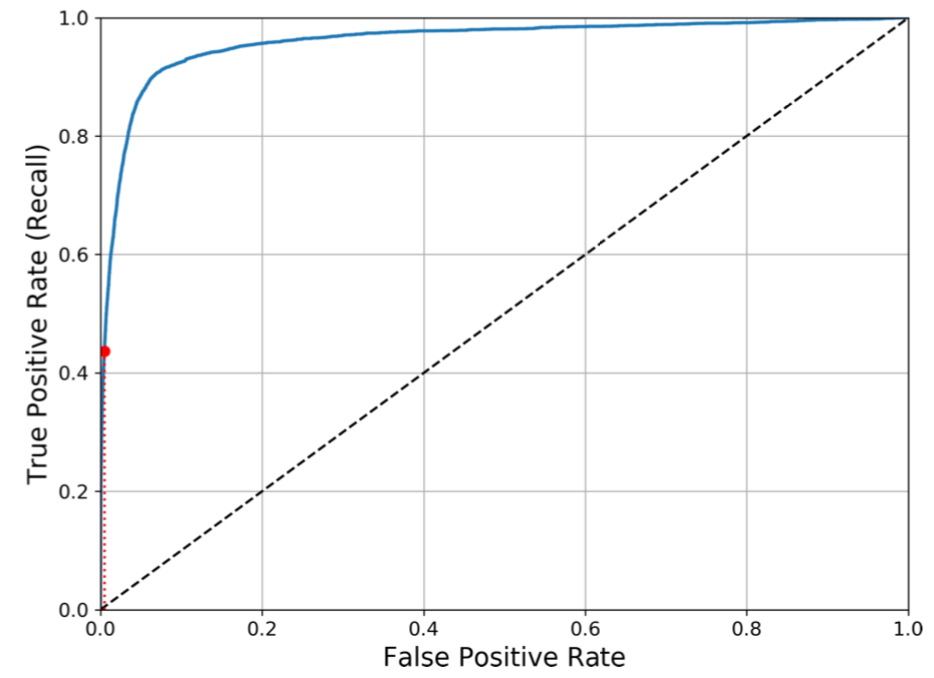
\includegraphics[width=0.3\textwidth]{note_images/ROC_curve.png} %插入图片,[]中设置图片大小,{}中是图片文件名
  \end{figure}

  y轴recall值,x轴false positive rate$FPR = \frac{FN}{FN + TN} = \frac{FN}{1-specificity}$

  期望的ROC curve为recall从0快速增长到1。并保持直到$FPR$为1。
  
  \quad 即期望曲线下方面积接近1\\
\textbf{learning curves}:观察模型是否有over underfit

  \begin{figure}[H] %H为当前位置,!htb为忽略美学标准,htbp为浮动图形
    \centering %图片居中
    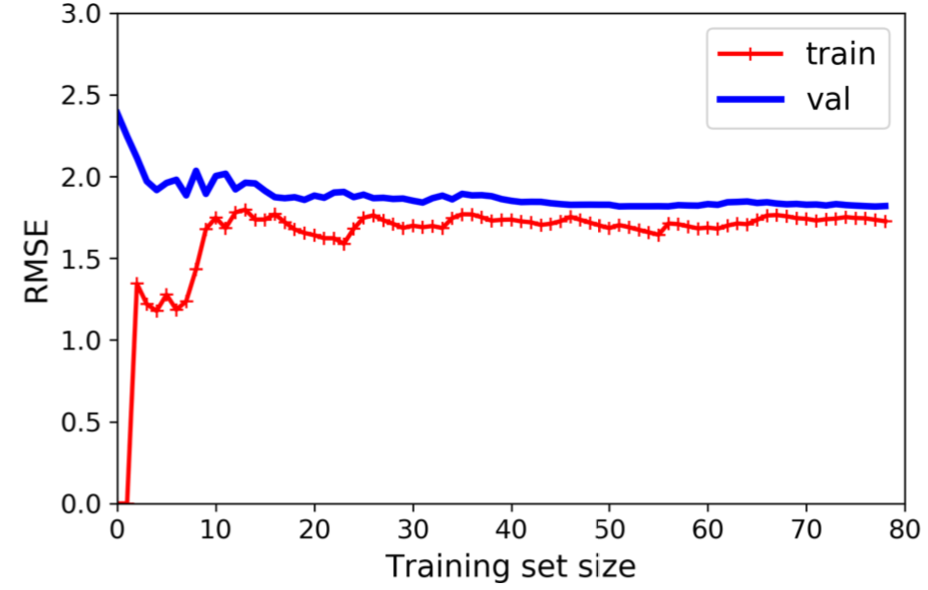
\includegraphics[width=0.3\textwidth]{note_images/learning_curve.png} %插入图片,[]中设置图片大小,{}中是图片文件名
  \end{figure}

  x轴为\textbf{一整次训练(包含多次epoch)使用的训练集大小},y轴为root MSE。

  画出训练集\ 测试集在使用不同训练集大小后的root MSE。

  分析:

  \quad 期望2曲线平缓值低且相近,

  \quad 当2曲线平缓值差值较大,测试集平缓值较低,则过拟合

  \quad 当2曲线平缓值较高,则欠拟合\\
\textbf{模型复杂度-error epoch-error}:

  \begin{figure}[H] %H为当前位置,!htb为忽略美学标准,htbp为浮动图形
    \centering %图片居中
    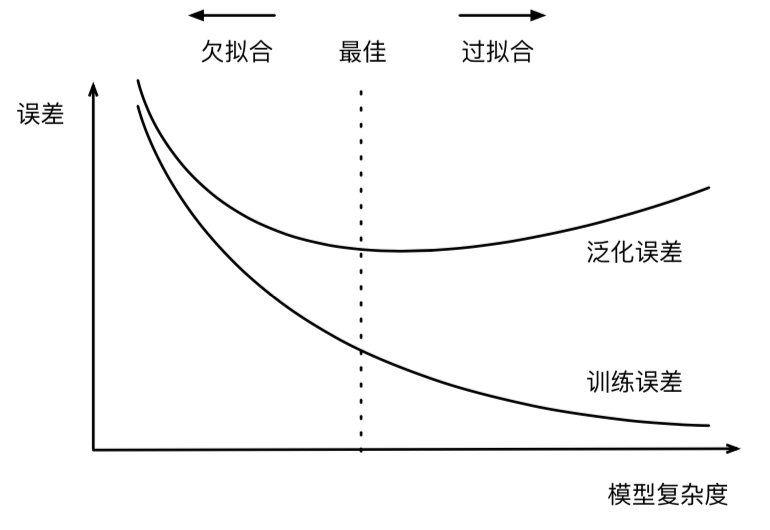
\includegraphics[width=0.3\textwidth]{note_images/epoch-complex-error.png} %插入图片,[]中设置图片大小,{}中是图片文件名
  \end{figure}

  2种图,形状类似,x轴内容不同\\

\end{document}
